\section{Mașini cu vector suport}

\subsection{Noțiuni generale}

Mașinile cu vector suport au devenit populare în ultimii ani pentru rezolvarea problemelor de clasificare sau regresie. Acestea realizează o clasificare de tip două clase prin folosirea modelului liniar de forma
\begin{align}
	y(x) = w^T\phi(x) + b
\end{align}
unde $\phi$ este o transformare a spațiului caracteristic.

Datele de antrenare sunt alcătuite din N vectori de intrare $x_1, ...,x_N$ fiecare dintre aceștia având asociate valorile $t_1, ...,t_N$ din mulțimea $t_n \in \{-1,1\}$, iar rezultatul din $y(x)$ reprezintă scorul asociat vectorului de intrare $x$.

De asemenea trebuie să ne asigură că în momentul antrenării setul de date este liniar separabil în spațiul caracteristicilor ceea ce înseamnă că pentru orice alegere a parametrilor $w$ și $b$ dacă funcția $y(x_n) > 0$ atunci valoarea asociată trebuie să fie $t_n = +1$. Situația este similară și pentru cazul în care $y(x_n ) < 0$, atunci valoarea asociată trebuie să fie $t_n = -1$. 
Concluzionând cele două proprietăți menționate anterior putem afirma faptul că următoarea inecuație trebuie să fie mereu validă  $t_n y(x_n) > 0$. 

Mașinile cu vector suport abordează problema prin conceptul de „margine” ce este definită ca fiind cea mai mică distanță dintre o frontieră de decizie și orice exemplu primit. O ilustrație a acestui fapt se poate vedea în figura 2.1.
\begin{figure}[!h]
	\centering
	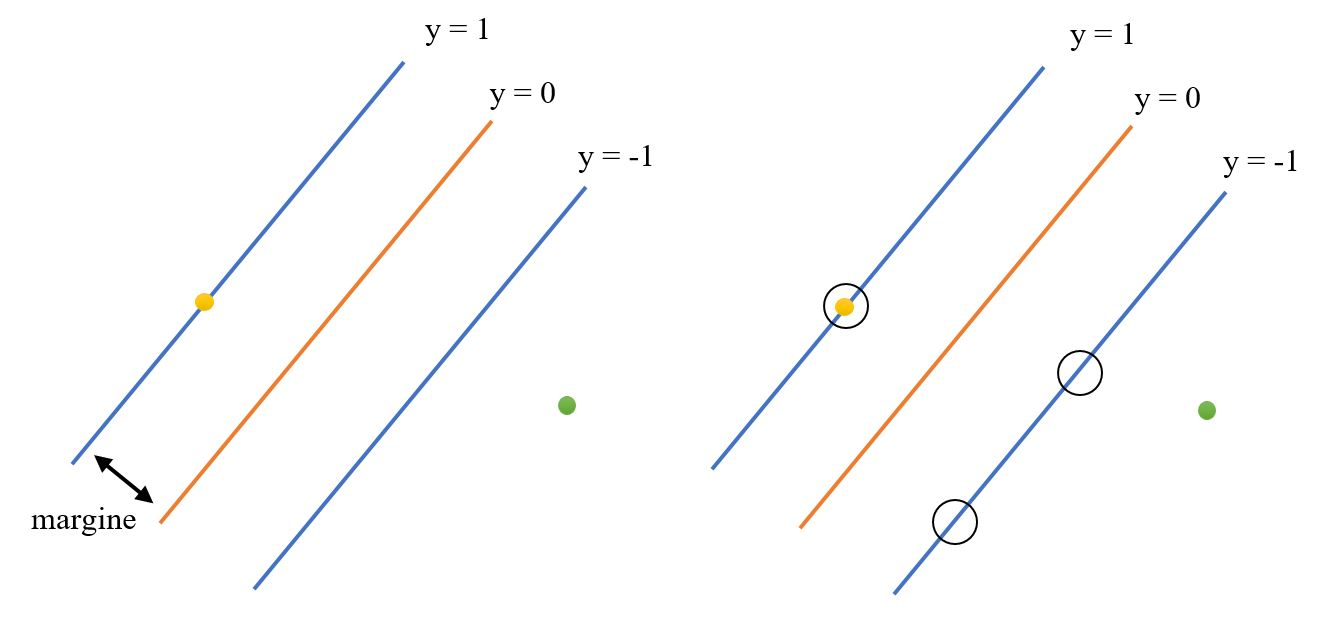
\includegraphics[max width=10cm,max height=10cm,keepaspectratio]{img_2_1}
	\caption[Mașini cu vector suport]{Marginea este definită ca distanța perpendiculara dintre limita de decizie și cel mai apropiat punct, după cum se poate observa în figura din stânga. Maximizăm limita marginii precum în figura din dreapta. Locația acestei limite este determinată de mașinile cu vectori suport indicate prin cercuri.}
\end{figure} 

În cazul mașinilor cu vectori suport, limita de decizie este aleasă să fie drept locația unde „marginea” este maximă. Această decizie este motivată de folosirea „teoriei computaționale de învățare” cunoscută drept „teoria statistică de învățare”. 

Primul model de distribuție peste vectorii de intrare $x$ pentru orice clasa folosește densitatea Parzen cu un nucleu Gaussian având parametrul comun $\sigma^2$. Utilizarea limitei optime determină cel mai bun hiperplan prin minimizarea probabilității de eroare relative densității modelului învățat. 

În cazul limitei $\sigma^2 \rightarrow 0$, hiperplanul optim este cel care are marginea maximă. Intuitiv, deoarece $\sigma^2$ este redus, hiperplanul este dominat mai mult de punctele din apropiere decât de cele din depărtare, în limită hiperplanul devenind independent de datele ce nu sunt mașini cu vector suport \hyperlink{ChristopherBishop}{[8]}. 

\subsection{Mașini cu vector suport multiclasă}

În principiu, mașinile cu vector suport sunt clasificatori de tip două clase însă, în practică întâlnim multe cazuri în care avem nevoie de probleme ce presupun mai mult de două clase. De-a lungul timpului au fost propuse diferite variante de rezolvare a problemei construcției mașini cu vector suport multiclasă.

Cea mai cunoscută abordarea (Vapnik, 1998) este reprezentată de construcția a K mașini cu vectori suport separate, unde în fiecare $k^{th}$  model, $y_k(x)$ este antrenat folosind date din clasa $C_k$ pe post de date de antrenare pozitive, iar datele din celelalte $K-1$ clase rămase pe post de date de antrenare negative. Această tehnică este cunoscută sub numele de „unul-versus-toți”. 

Astfel noile predicții pentru un input $x$ for fi făcute pe baza următoarei relații
\begin{align}
	y(x) = \max_{\substack{k}}y_k(x)
\end{align}

Evident, în această abordare pot apărea anumite probleme precum cea legată de faptul că acești clasificatori au fost antrenați pe diferite clase, ceea ce înseamnă că nu avem neapărat o garanție a faptului că se vor comporta în practică pe tipuri diferite de intrări similar cu datele de antrenare.

O altă problemă întâlnită în această abordare de unu-versus-toți este legată de cantitatea datelor de antrenare în sensul de pierdere al echilibrului dintre exemplele pozitive și cele negative. Spre exemplu, să presupunem că avem 10 tipuri de clase. Pentru o instanță a unei mașini cu vector suport vom avea $10\%$ dintre toate datele de antrenare disponibile încadrate precum exemple pozitive, iar cealaltă parte, mult mai densă, de $90\%$ vor reprezenta exemple de antrenare negative, fapt ce va crea o discrepanță foarte mare între ele, astfel simetria fiind pierdută.

Weston and Watkins (1999) definesc o singură funcție obiectiv pentru antrenarea tuturor celor $K$ vectori suport mașină simultan, acest procedeu fiind bazat pe maximizarea marginilor pentru fiecare clasă. Acest lucru produce un efect de rulare înceată a antrenării deoarece rezolvarea a $K$ probleme separate de optimizare ar însemna că pentru fiecare $N$ punct de date are un cost de rulare per total de $O(KN^2)$, iar o singură problemă de optimizare cu dimensiunea $(K - 1)N$ poate fi rezolvată cu un cost total de $O(K^2N^2)$.

Una dintre cele mai întâlnite metode de rezolvare a acestor probleme este o abordare în care vom antrena $K(K-1)/2$ vectori suport mașină diferiți pentru toate perechile de clase posibile, iar rezultatul final va fi determinat de aceea mașină cu vector suport care va răspunde cu un număr cât mai mare de voturi (scor) dintre toate cele $K(K-1)/2$ posibilități. Această este numită deseori drept o antrenare „unu-versus-unu”. Evident, în această situație timpul de rulare va crește odată cu numărul claselor pentru care trebuie antrenate mașinile cu vector suport.

Pentru a rezolva această problemă a timpului de execuție putem organiza perechile de clasificare într-un graf aciclic. Astfel, pentru K clase pe care le avem de analizat vom avea în total $K(K-1)/2$ vectori suport mașină, iar pentru a clasifica o intrare vom avea nevoie doar de $K-1$ perechi de clasificatori spre a fi evaluați cu clasificatorii specifici traversări grafului.

O abordare diferită a clasificării multiclasă în cazul mașinilor cu vectori suport, bazată pe coduri de ieșire corectoare de erori dezvoltate de Dietterich și Bakiri (1995) și ulterior aplicate pe mașini cu vector suport de către Allwein, Schapire și Singer (2000). 
Acest lucru poate fi văzut precum o generalizare a schemei de vot unu-versus-unu în care cele mai generale părți ale clasei sunt folosite pentru formarea de clasificatori individuali.
Cele $K$ clase sunt representate precum seturi particulare de răspunsuri provenite din clasificatori de două clase, iar împreună cu o schemă de decodare potrivită oferă robustețe la erori și la ambiguitatea rezultatelor clasificatorilor individuali.

Deși clasificarea cu mașini vectori suport multiclasă încă are multe capitole de îmbunătățit, în practică abordarea unul-versus-toți rămâne cea mai utiliza în ciuda limitărilor de performanță aferente \hyperlink{ErinAllweinRobertSchapireYoramSinger}{[9}, \hyperlink{JasonWestonSimonWatkins}{10}, \hyperlink{ThomasDietterichGhulumBakiri}{18}, \hyperlink{VladimirVapnik}{19]}.

\subsection{Mașini cu vector suport pentru regresie}

În regresia liniară simplă se minimizează o funcție de eroare regularizată definită de
\begin{align}
	\frac{1}{2}\sum_{n=1}^{N}\{y_n-t_n\}^2+\frac{\lambda}{2}\norm w^2
\end{align}

Pentru a obține soluțiile, funcția cuadrică de eroare va fi înlocuită de o funcție numită $\epsilon$ - funcție de eroare intensivă (Vapnik, 1995) ce ne returnează eroarea 0 dacă diferența absolută dintre predicția $y(x)$ și asocierea sa $t$ este mai mică decât $\epsilon$ unde $\epsilon > 0$. Un exemplu simplu de $\epsilon$ - funcție de eroare intensivă cu un cost liniar asociat cu eroarea din exteriorul regiunii este
\begin{align}
	E_{\epsilon}(y(x) - t) = 
	\begin{cases}
	0,& \text{dacă } \abs {y(x) - t} < \epsilon\\
	\abs {y(x) - t} - \epsilon,              & \text{altfel}
	\end{cases}
\end{align}
exemplu ilustrat în figura 2.2.
\begin{figure}[!h]
	\centering
	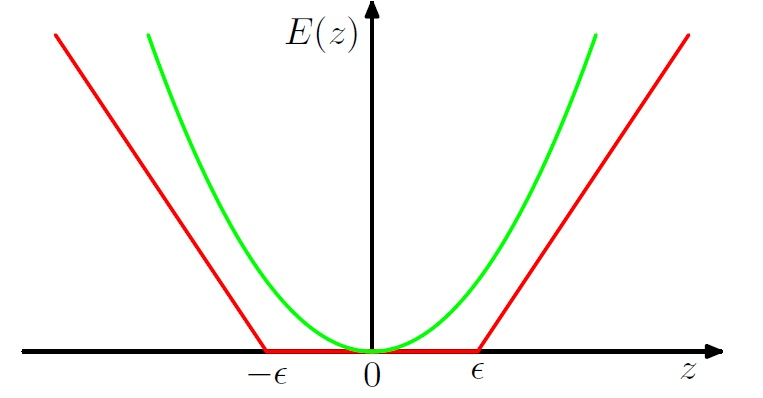
\includegraphics[max width=10cm,max height=10cm,keepaspectratio]{img_2_2}
	\caption[Mașini cu vector suport pentru regresie]{Cu roșu se poate observa $\epsilon - functie de eroare intensivă$, iar cu verde se poate observa o funcție cuadrică de eroare. Imagine preluată din \hyperlink{ChristopherBishop}{[8]}.}
\end{figure}
 
Prin urmare, vom minimiza o funcție de eroare regularizata dată prin
\begin{align}	
	C\sum_{n = 1}^{N}E_{\epsilon}(y(X_n) - t_n) + \frac{1}{2}\norm w ^ 2
\end{align}

Similar cu cele prezentate anterior putem alege un prag $\xi_n \geq 0$ și $ \widehat{\xi_n} \geq 0$, unde $\xi_n > 0$ corespunde punctului pentru care următoare condiție este îndeplinită $t_n > y(x_n) + \epsilon$, iar  $ \widehat{\xi_n} \geq 0$ corespunde punctului pentru care următoarea condiție este îndeplinită $t_n < y(x_n) - \epsilon$. Acestea fiind ilustrate în figura 2.3.
\begin{figure}[!h]
	\centering
	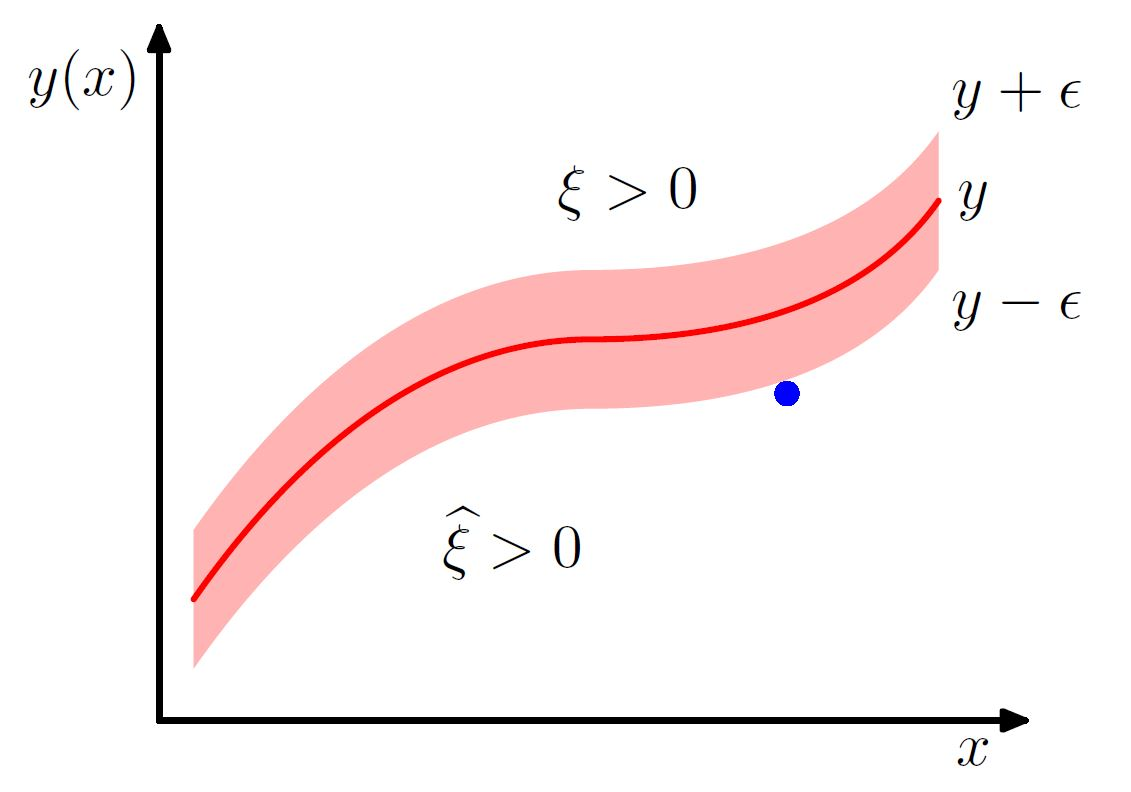
\includegraphics[max width=10cm,max height=10cm,keepaspectratio]{img_2_3}
	\caption[Mașini cu vector suport pentru regresie 2]{Este prezentată o regresie vector suport mașină evidențiind curba de regresie împreună cu zona $\epsilon – intensiv$. De asemenea, sunt prezentate variabilele $\xi$ și $ \widehat{\xi}$. Punctele de deasupra zonei $\epsilon$ au $\xi > 0$ și $ \widehat{\xi} = 0$, iar punctele de sub zona $\epsilon$ au $\xi = 0$ și $ \widehat{\xi} > 0$, în cele din urmă, punctele din interiorul zonei $\epsilon$ au $\xi = 0$ cât și $ \widehat{\xi} = 0$. Imagine preluată din \hyperlink{ChristopherBishop}{[8]}.}
\end{figure}

Condiția ca un punct să fie în interiorul zone $ \epsilon $ este ca $y_n - \epsilon \leq t_n \leq y_n + \epsilon$ unde $y_n = y(x_n)$. Introducând variabilele $\xi_n$ și $\widehat{\xi_n}$ permitem punctelor să se afle în afara zonei de interes condiționat de faptul că variabilele introduse sunt nenule iar următoarele condiții sunt indeplinite
\begin{align}	
	t_n \leq y(x_n) + \epsilon + \xi_n
\end{align}
\begin{align}	
	t_n \geq y(x_n) - \epsilon - \widehat{\xi_n}
\end{align}

În practică, în detrimentul fixării unui parametru $\epsilon$ se preferă fixarea unui parametru $v$ ce are drept rol principal limitarea punctelor din afara zonei $\epsilon$. O rezolvare a unei probleme de regresie având un set de date sinusoidal cu vectori suport mașină este ilustrată în figura 2.4. În această situație parametrii $v$ și $C$ au fost aleși manual, însă în practică aceste valori sunt determinate automat \hyperlink{ChristopherBishop}{[8]}.
\begin{figure}[!h]
	\centering
	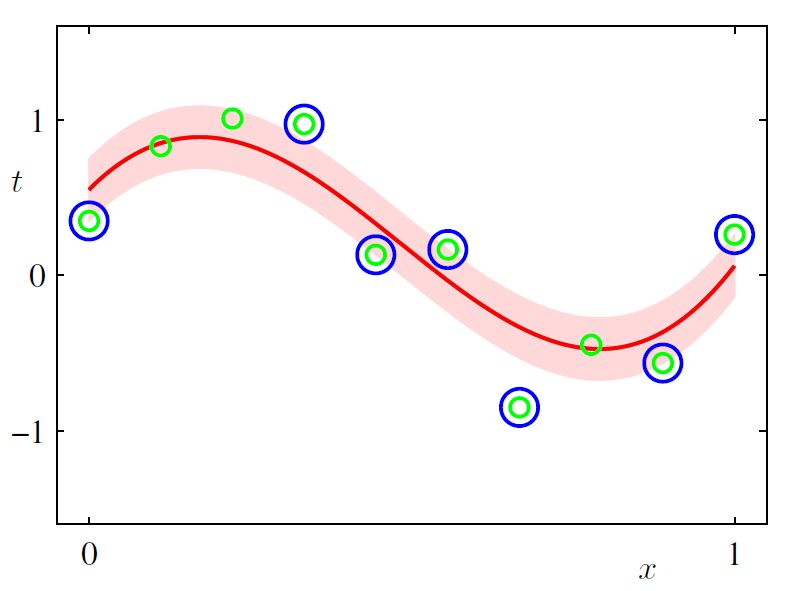
\includegraphics[max width=10cm,max height=10cm,keepaspectratio]{img_2_4}
	\caption[Mașini cu vector suport pentru regresie 3]{Este prezentată un vector suport mașină pentru regresie aplicat pe un set de date sinusoidal și utilizând un nucleu Gaussian. Curba de regresie prezisă este ilustrată prin linia roșie, iar zona $\epsilon - intensiv$ este ilustrată prin zona roșie hașurată. Datele sunt indicate prin cercurile verzi, iar vectorii suport mașină sunt indicați prin cercurile albastre. Imagine preluată din \hyperlink{ChristopherBishop}{[8]}.}
\end{figure}

\section{Histograme de gradienți orientați}

\subsection{Noțiuni generale}

Histograma de gradienți orientați este un descriptor utilizat în vederea artificială și în procesarea imaginilor cu scopul de a detecta obiecte. 

Prin această tehnică se numără aparițiile orientării gradientului în anumite porțiuni localizate ale imaginii.

Ideea principală ce stă la baza histogramei de gradienți orientați este reprezentată de faptul că aspectul și forma obiectului dintr-o imagine pot fi descrise prin distribuirea intensității gradienților sau a muchiilor direcțiilor. În figura 2.5 este prezentat un exemplu practic.
\begin{figure}[!h]
	\centering
	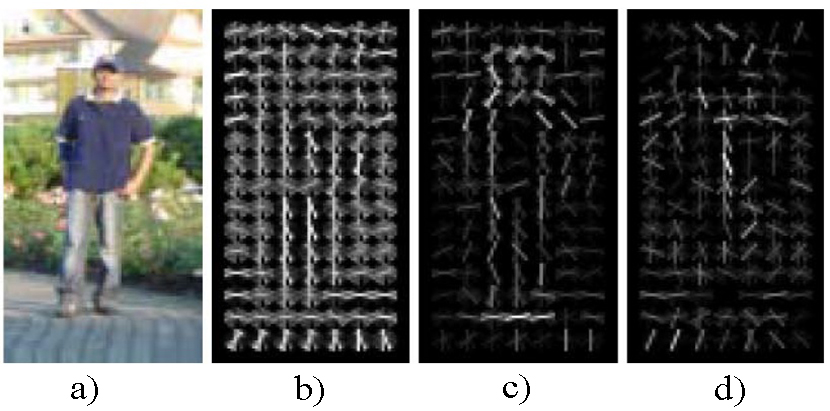
\includegraphics[max width=10cm,max height=10cm,keepaspectratio]{img_2_5}
	\caption[Descriptor HOG]{(a) imaginea originală; (b) descriptorul histogramei de gradienți orientați asociate imaginii; (c) valorile pozitive din $w$ a descriptorul histogramei de gradienți orientați asociate imaginii; (d) valorile negative din $w$ a descriptorul histogramei de gradienți orientați asociate imaginii. Imagine preluată din \hyperlink{NavneetDalalBillTriggs}{[12]}.}
\end{figure}

Imaginea este împărțită în mici regiuni conectate numite celule, iar pentru pixelii din fiecare celulă se obține o histogramă de gradienți orientați. Descriptorul este rezultatul concatenării acestor histograme. Se poate îmbunătății acuratețea prin normalizarea histogramelor, această normalizare are ca rezultat o invarianță mai bună a schimbărilor intensităților luminii sau apariției umbrelor. În figura 2.6 sunt reprezentate vizual aceste noțiuni.
\begin{figure}[!h]
	\centering
	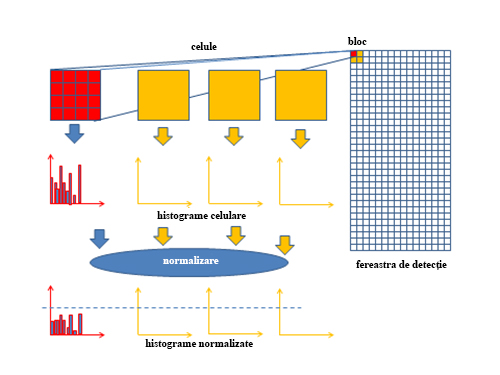
\includegraphics[max width=10cm,max height=10cm,keepaspectratio]{img_2_6}
	\caption{Procesul de extragere a histogramelor de gradienți orientați}
\end{figure}

Histogramele de gradienți orientați prezintă principalul avantaj prin faptul că lucrează la nivel de celulă locală, astfel, în practică, se comportă bine la invarianța geometrică și transformările fotometrice, exceptând, desigur, orientarea obiectului \hyperlink{RichardSzeliski}{[13]}. 

\subsection{Etapele metodei}

\subsubsection {Compunerea gradientului}

Principalul pas în majoritatea determinării de caracteristici în preprocesarea de imagini este de a asigura o normalizarea a valorilor aspura culorii. Astfel, primul pas constă în determinarea valorii gradienților, iar cea mai comună metodă pentru a face acest lucru este să aplicăm un filtru $1-D$ centrat, atât pe direcția verticală cât și pe direcția orizontală. Pentru acest lucru se pot utiliza următoarele nuclee de filtre
\begin{align}	
	[-1, 0, 1]  \quad sau  \quad  [-1, 0, 1]^T
\end{align}

\subsubsection {Orientarea binară}

În continuare trebuie create histogramele de celule. Fiecare pixel dintr-o celulă primește un vot ponderat pentru o poziție pe un canal orientat al histogramei. Canalele histogramei sunt distribuite uniform intre 0 și 180 de grade sau intre 0 și 360 de grade. În practică, pentru a determina contribuția pixelilor se folosește magnitudinea gradientului.

\subsubsection {Blocurile descriptor}

Datorită diferitelor situații în care iluminarea și contrastul pot varia, este nevoie de normalizarea locală a gradientului, ceea ce presupune gruparea celulelor în blocuri mai mari, iar ulterior concatenarea mai multor blocuri formează descriptorul histogramei de gradienți orientați.

\subsubsection {Normalizarea blocului}

În ceea ce privește normalizarea blocurilor putem folosi mai multe metode propuse de Dalal și Triggs. În continuare vom presupune că $v$ este vectorul ce nu este normalizat și ce conține histogramele, $\norm{v}_k$ reprezintă norma vectorului, pentru $k = 1,2$ la care adugăm și o constantă $e$. Din acestea deducem următoarele forme de normalizare
\begin{align}	
	L2-norm: f = \frac{v}{\sqrt{\norm{v}_2^2 + e^2}}
\end{align}
\begin{align}	
	L1-norm: f = \frac{v}{\norm{v}_1 + e}
\end{align}
\begin{align}	
	L1-sqrt: f = \sqrt{\frac{v}{\norm{v}_1 + e}}
\end{align}
Toate aceste metode de normalizare oferă o îmbunătățire semnificativă făță de datele nenormalizate, iar cea care pare a se comporta puțin mai bine în detrimentul celorlalte este $L1-norm$.

\subsubsection {Clasificarea cu suport vector mașină}

Pasul final în procesul de detecție folosind histogramele de gradienți orientați este de a antrena clasificatori cu descriptorii obținuți. Clasificarea cu vectori suport mașină poate fi o variantă.

\subsubsection {Clasificarea cu rețele neuronale}

În cazul în care se dorește o acuratețe de clasificare mai bună se pot folosi rețele neuronale în detrimentul vectorilor suport mașină \hyperlink{NavneetDalalBillTriggs}{[12]}.

\section{Metoda glisării ferestrei}

\subsection{Noțiuni generale}

Tehnica de glisare a ferestrei este una des întâlnită în detectarea de obiecte în imagini. Aceasta presupune deplasarea ferestrei pe toată suprafața imaginii cu un anumit salt de pixel stabilit în prealabil. De asemenea, această tehnică poate fi folosită pentru diferite dimensiuni de detecție. Astfel avem ca alternative, fie să mărim sau să micșorăm dimensiunea ferestrei glisante, fie să mărim sau să micșorăm dimensiunea imaginii și să rulăm aceeași dimensiune a ferestrei pe diferite dimensiuni ale imaginii \hyperlink{RichardSzeliski}{[13]}.

Tehnica prezentată anterior este ilustrată și în figura 2.7 sau în figura 2.8
\begin{figure}[!h]
	\centering
	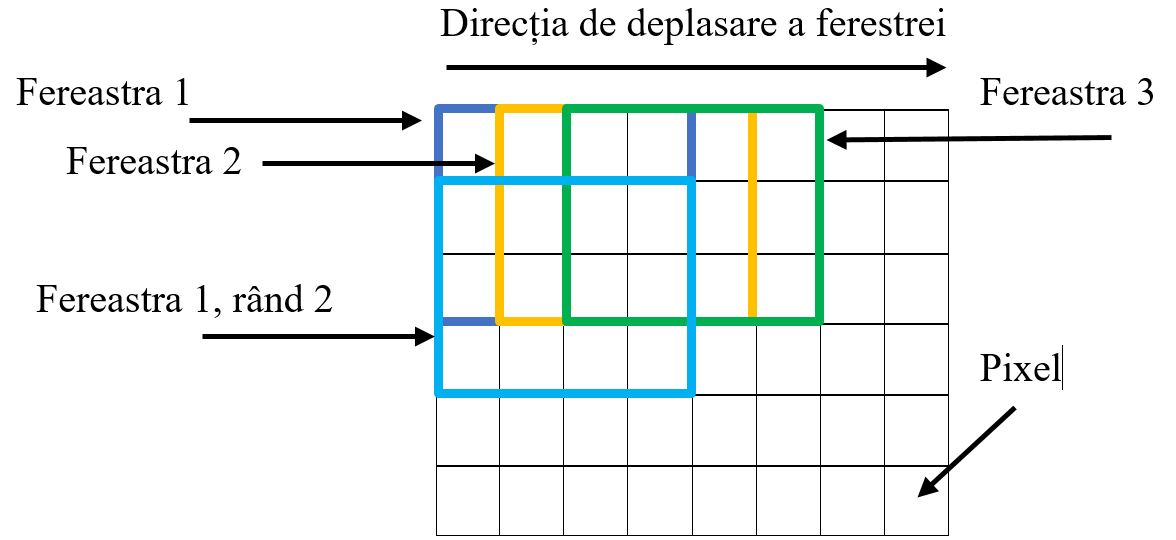
\includegraphics[max width=10cm,max height=10cm,keepaspectratio]{img_2_7}
	\caption{Metoda glisării ferestrei la nivel de concept}
	\label{fig:nonfloat}
\end{figure}
\begin{figure}[!h]
	\centering
	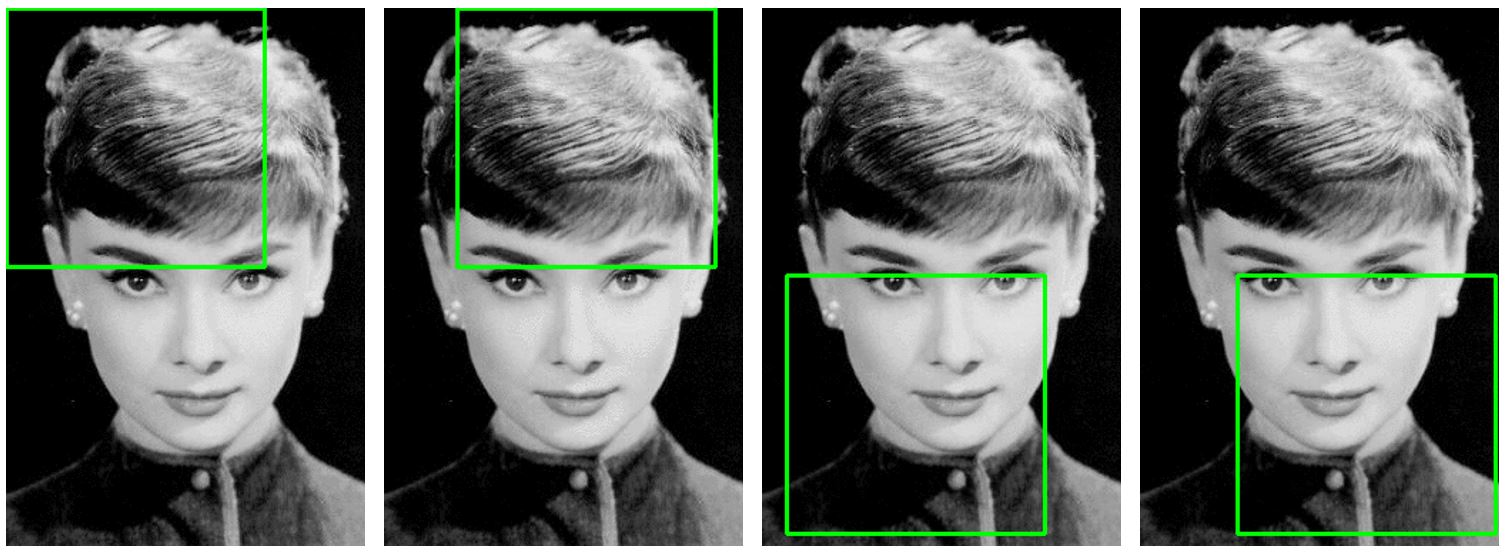
\includegraphics[max width=15cm,max height=15cm,keepaspectratio]{img_2_8}
	\caption{Metoda glisării ferestrei în practică, în patru momente diferite}
	\label{fig:nonfloat}
\end{figure}

\section{IPM (Inverse Perspective Mapping)}

\subsection{Noțiuni generale}

IPM-ul reprezintă o tehnică de transformare geometrică care proiectează fiecare pixel a unui obiect din 3D într-o perspectivă 2D. Acest lucru înseamnă repoziționarea fiecărui pixel într-o poziție nouă corespunzătoare noii perspective, astfel construindu-se noua imagine. Din punct de vedere matematic acest lucru poate fi descris printr-o proiecție din planul Euclidian 3D de forma $W = \{(x,y,z)\} \in E^3$ într-un plan 2D de forma $I = \{(u,v)\} \in E^2$. Această transformare mai poartă numele și de „Bird's eye view” datorită privirii de sus pe care o oferă asupra imaginii originale. În figura 2.9 este prezentat vizual acest model.

\begin{figure}[!h]
	\centering
	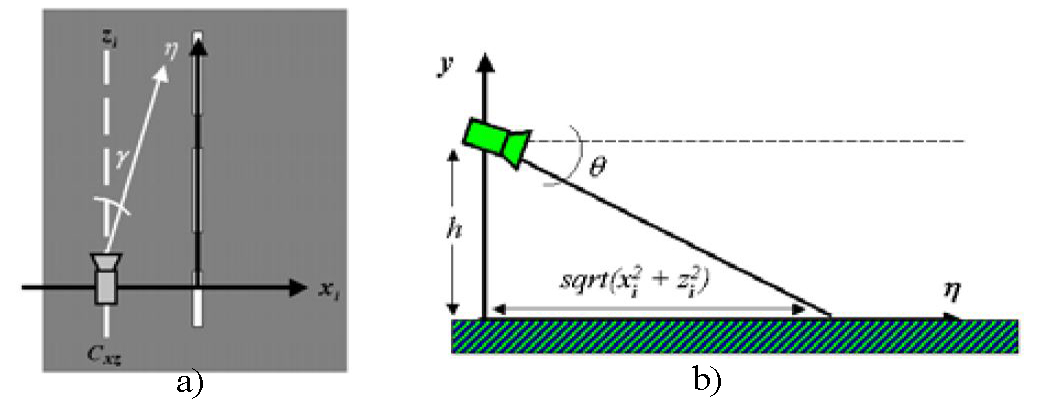
\includegraphics[max width=15cm,max height=15cm,keepaspectratio]{img_2_9}
	\caption[Modelul IPM]{a) vizualizarea geometrică „de sus” în planul construit; b) vizualizarea geometrică din lumea reală. Imagine preluată din \hyperlink{AnuarMikdadMuadAiniHussainSalinaAbdulSamadMohdMarzukiMustaffaBurhanuddinYeopMajlis}{[1]}.}
	\label{fig:nonfloat}
\end{figure}

Pentru aflarea coordonatelor în noul plan putem folosi următoarele formule 2.12 și 2.13 rezultate pe baza modelului IPM.

\begin{align}	
	u(x,0,z) = \frac{\gamma(x,0,z) - (Y-\alpha)}{\frac{2\alpha}{n-1}}
\end{align}
\begin{align}	
	v(x,0,z) = \frac{\theta(x,0,z) - (\Theta - \alpha)}{\frac{2\alpha}{m-1}}
\end{align}

În formulele prezentate au fost folosite:

$\gamma = tan^{-1}(\frac{z}{x})$;

$\theta = tan^{-1}(\frac{h}{\sqrt{x^2+z^2}})$;

$Y$ - reprezintă unghiul dintre proiecția axei optice pe planul real; 

$\Theta$ - reprezintă unghiul dintre proiecția axei optice și planul orizontal;
 
$\alpha$ - reprezintă unghiul de înclinație al camerei;

$m \times n$ reprezintă rezoluția imaginii.

În figura 2.10 se poate observa un exemplu practic al IPM-ului.

\begin{figure}[!h]
	\centering
	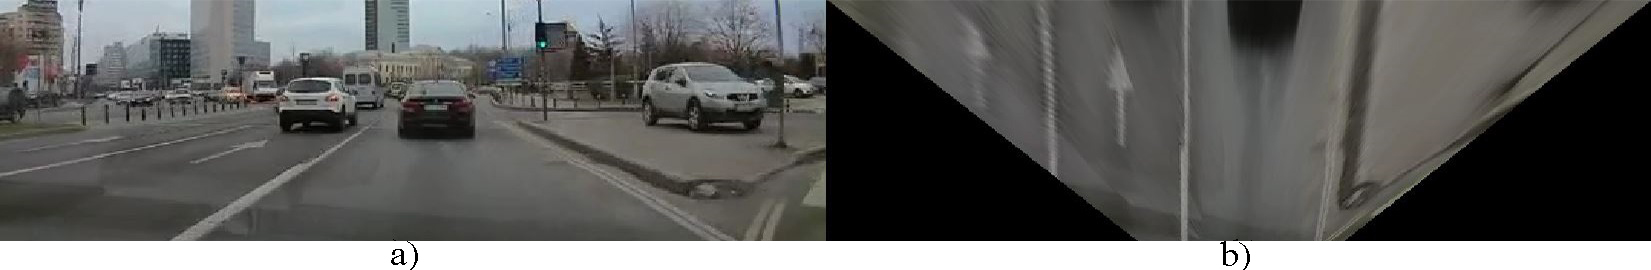
\includegraphics[max width=17cm,max height=17cm,keepaspectratio]{img_2_10}
	\caption[Imagine IPM]{Imaginea IPM (b) asociată unei imaginii din plan real (a).}
	\label{fig:nonfloat}
\end{figure}

Evident, formulele prezentate anterior prezintă un dezavantaj datorită faptului că procesarea prin intermediul lor se face pixel cu pixel. În elaborarea lucrării practice au fost folosite metode de obținere a IPM-ului mult mai rapide pentru a îndeplini unul dintre obiectivului lucrării și anume rularea în timp real a aplicației.

\begin{figure}[!h]
	\centering
	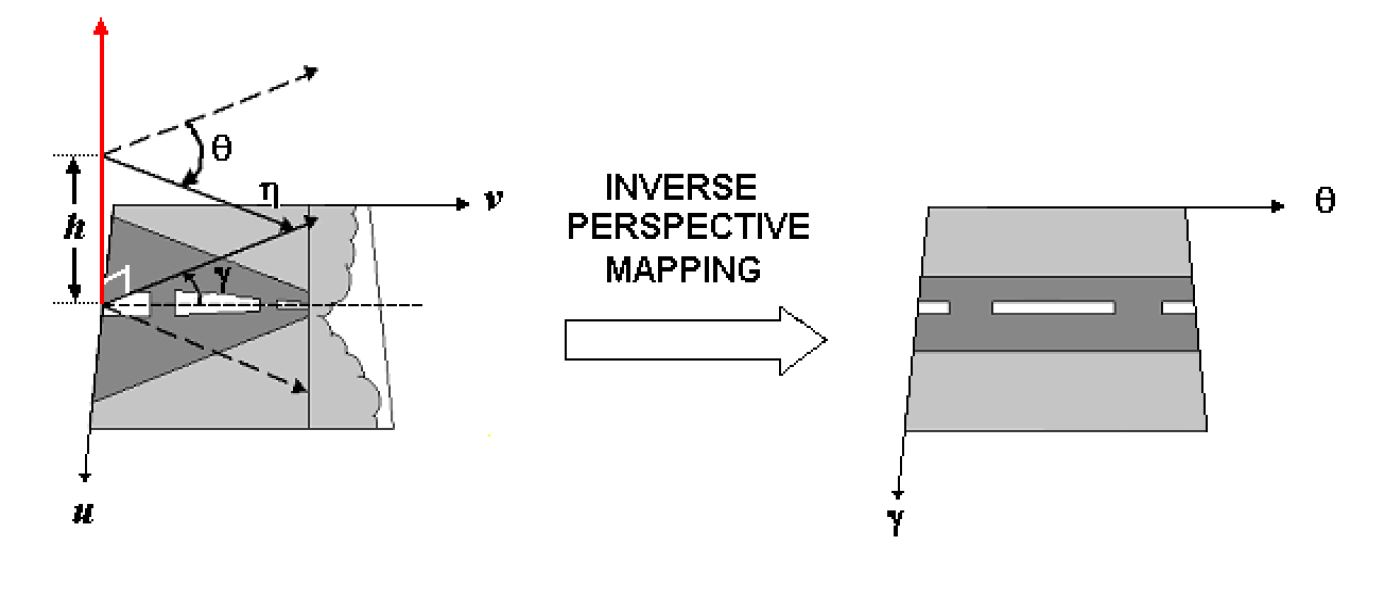
\includegraphics[max width=17cm,max height=17cm,keepaspectratio]{img_2_11}
	\caption[Reprezentare grafică IPM]{Reprezentarea grafică a IPM. Imagine preluată din \hyperlink{AnuarMikdadMuadAiniHussainSalinaAbdulSamadMohdMarzukiMustaffaBurhanuddinYeopMajlis}{[1]}.}
	\label{fig:nonfloat}
\end{figure}